%!TEX root = ../../thesis.tex

\section{World properties}
\label{chapter:limitations:wordlproperties}

\question{How the world properties (symmetries, size, \ldots) affect the learning properties?}

As discussed in section~\ref{chapter:lfui:symmetries}, the properties of the world can affect the learning performances. For example some worlds have symmetric properties which makes some tasks impossible to differentiate.

In this section, we compare how various planning methods perform on two different worlds, namely the pick and place scenario and the grid world. We investigate the performance of planning using a random strategy, several $\epsilon$-greedy methods, a strategy based on the task uncertainty (where we do not take the signal to meaning mapping uncertainty in to account), and our uncertainty based method described in chapter\ref{chapter:planning}. We will see that the size of the worlds and the properties of optimal policies impact the performance of these planning methods.

\subsection{Hypothesis and world properties}

We hypothesized that differences in the properties of each world will impact the performances of several planning methods, especially the random method and the e-greedy methods which are blind to the problem properties.

In the coming analysis, we consider three different world instances, a 5 by 5 grid world, a 25 by 25 grid world and the pick and place world of chapter~\ref{chapter:lfui}. In the following we present the main differences between these worlds.

First testing our planning method on a 5x5 and 25x25 allows to test how the size of the world influence the performances and to verify that our uncertainty measure is robust to such change. The main hypothesis is that the random action selection method will not scale well to this change in dimensionality. Indeed, in a 5x5 grid, taking random actions allows to explore the state space quite uniformly in a small number of steps, however in a 25x25 grid (625 states) the robot is unlikely to visit useful states given a limited number of iterations.

We choose to use a 25x25 grid because the resulting number of states (625) is almost equal to the number of states of the pick and place scenario (624), which allows to remove the size effects when comparing those two scenarios. By comparing the grid world and the pick and place scenario, we aim at investing how the maze like properties of the pick and place world compares with the more simple structure of the grid world. For the pick and place scenario, to reach the correct cubes' configuration the robot must achieve a very specific sequence of action in the correct order. As for a maze, only one correct path can be followed, however for the grid world a multitude of path can be chosen.

\todo{The ``maze like'' property can be measure by the amount of overlap between the optimal policies associated to two ``close'' task. For the pick and place scenario, if the signal to meaning mapping were known, to differentiate between two cube configuration that are close together, the agent must go towards those configuration to be able to discard one or an other task. For example, in our illustration of Figure~\ref{fig:lfui:pickplacesequence}, to differentiate between the two first state, one as to reach one of those two states to tell the identify the correct one. Indeed, their corresponding optimal policies are similar for every state except their two final states, i.e. both tasks share the same policies for 622 states our of 624. However for the grid world scenario, if the signal to meaning mapping were known, one could differentiate between the top right state and the state directly on the left of that top right state by simply performing a left action on the bottom right state. And this whatever the size of the grid. The optimal policies of those two task differs for all states along the two columns on the left of the grid, i.e. both tasks share the same policies for only 575 states our of 625 in our 25x25 grid world.}

\subsection{Method}

We used the same conditions as used in chapter~\ref{chapter:planning}, where the teacher is providing instructions following the feedback frame but we use only two dimensional signals of very good quality (i.e. between 90 and 100 percent of classification rate).

We simulated 50 runs of 100 iterations for each planning methods and each world considered. There where 10 steps of initialization before the agent starts computing the first likelihood. During the first 10 steps, the agent where acting randomly for all methods.

\subsection{Results}

In this subsection, we analyze the Figure~\ref{fig:wordlpropertiestimefirst} which displays the number of iterations needed to reach the first task with confidence. We first comment the difference between the 5x5 grid world and the 25x25 grid world, and then compare the grid world and the pick and place scenario.

\begin{figure}[!htbp]
\centering
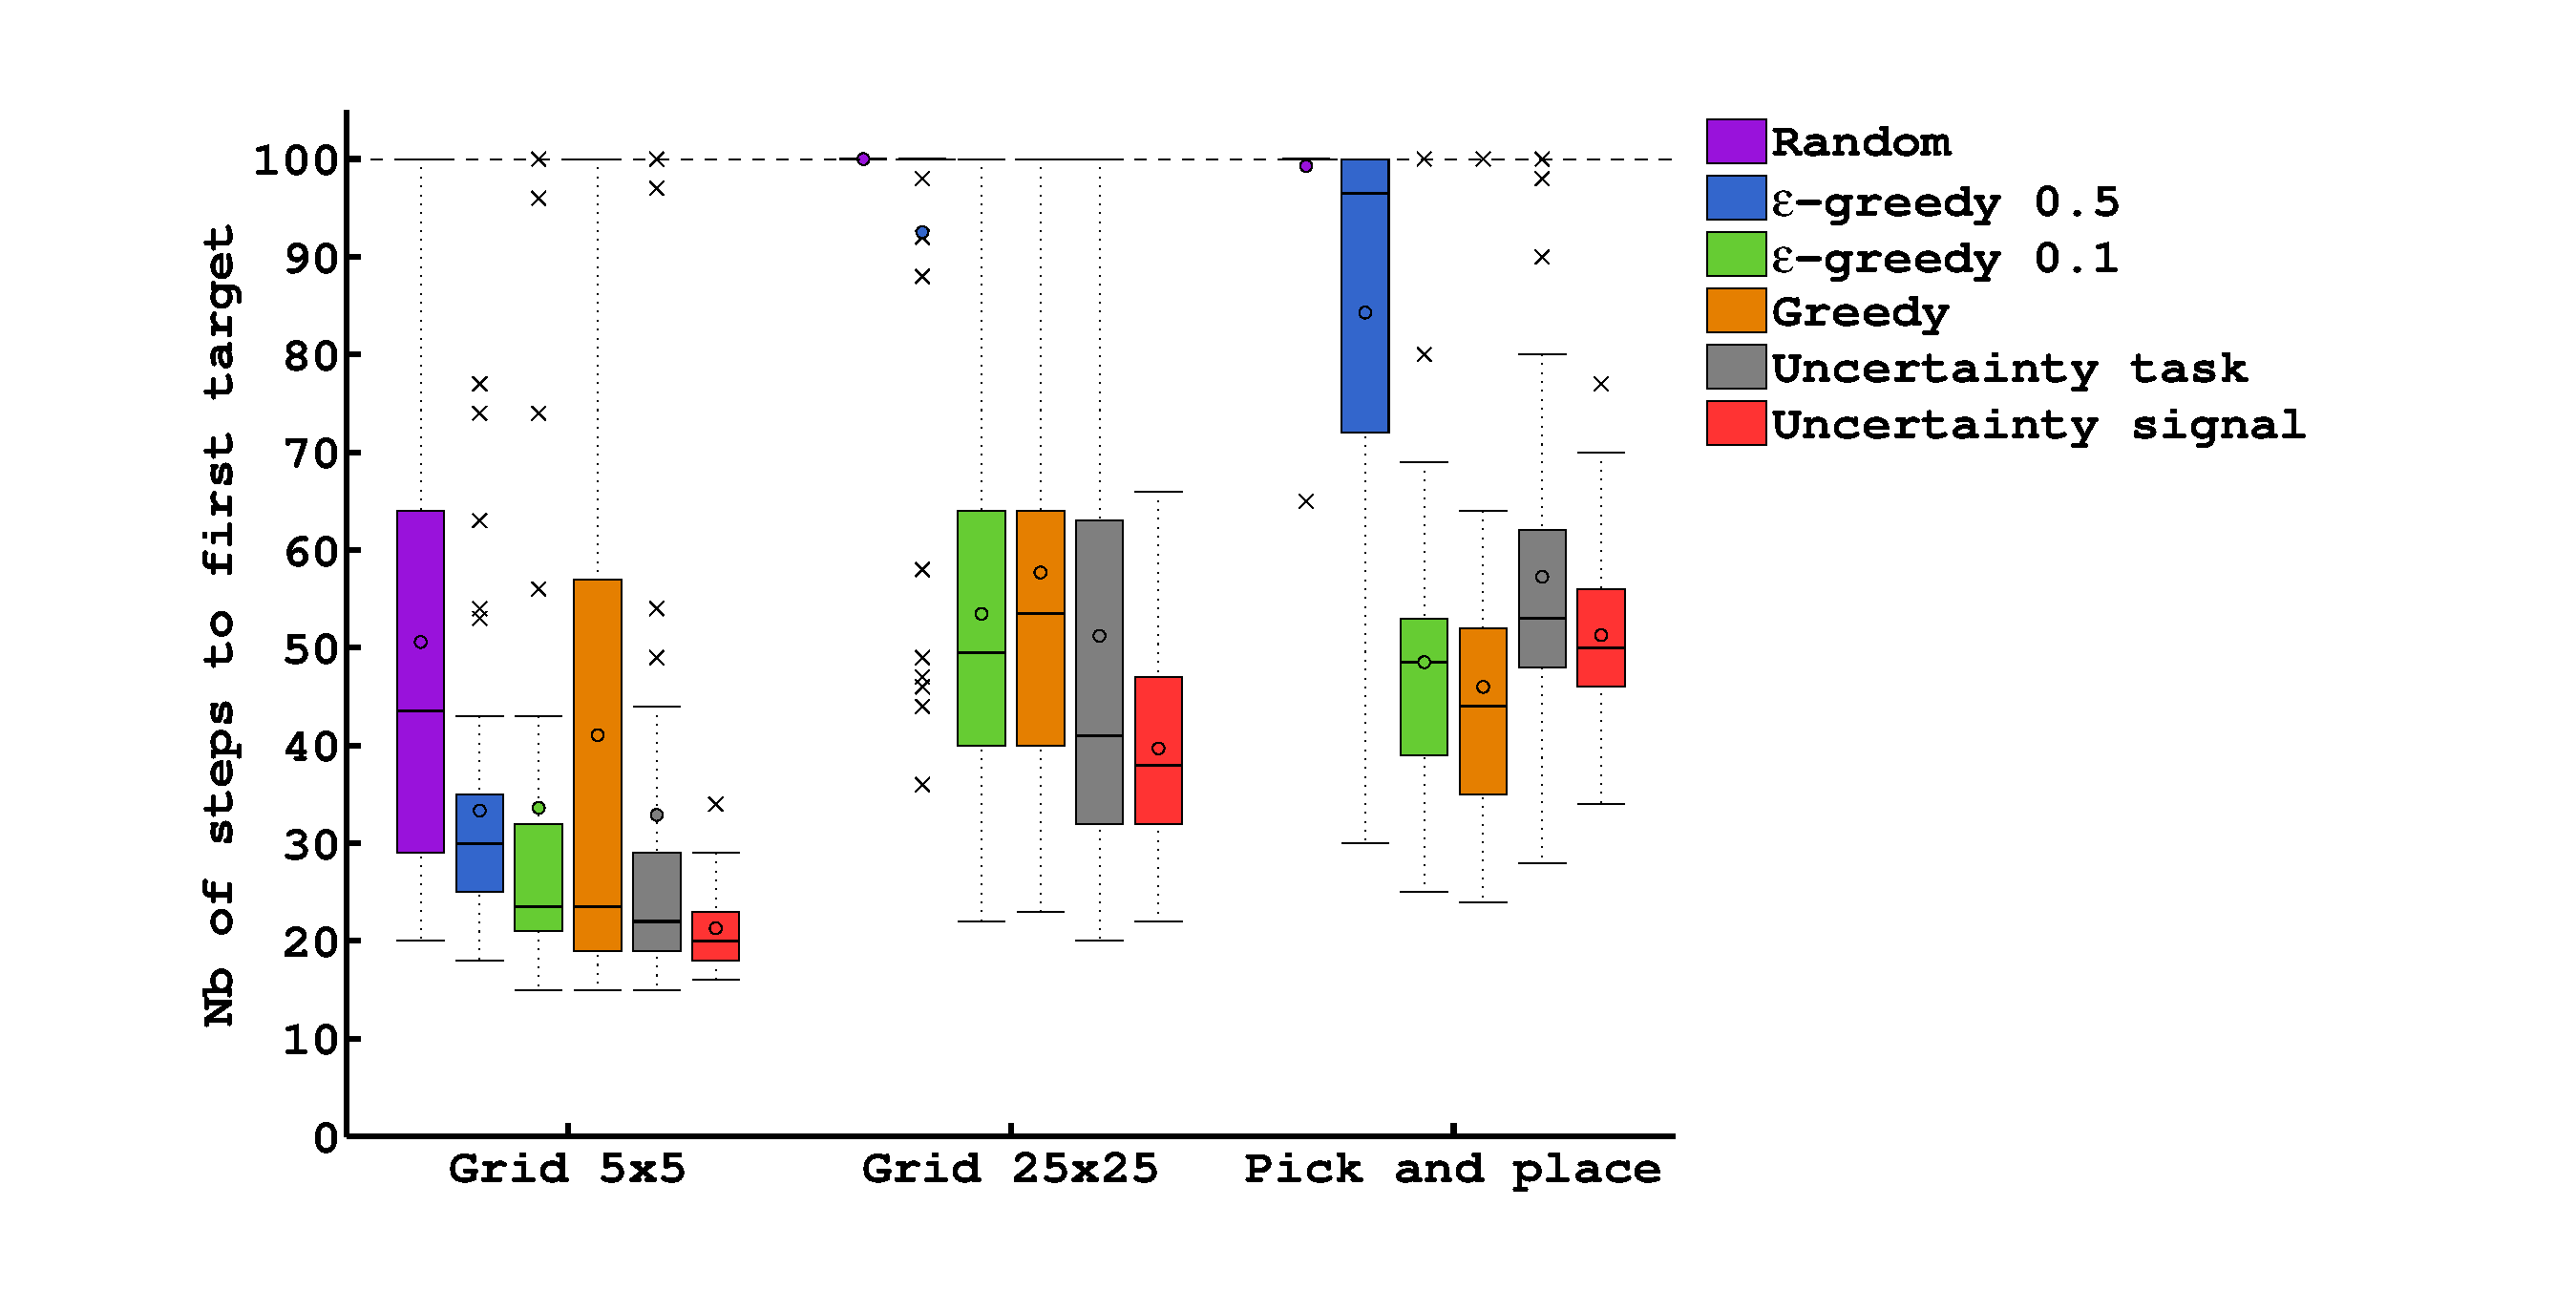
\includegraphics[width=\legendsidesize\columnwidth]{\imgpath/world_properties/firstreach.eps}
\caption{Number of steps needed to reach the first target state with confidence. When the dimensionality of the world increase, selecting actions randomly does not allow to identify any task in 100 iterations. Our uncertainty based method (uncertainty signal), is the most efficient at reaching the first task in the grid world scenarios but seems outperformed by a simple greedy approach in the pick and place scenario.}
\label{fig:wordlpropertiestimefirst}
\end{figure}

There is several aspects to keep in mind when analyzing Figure~\ref{fig:wordlpropertiestimefirst}. First, it displays the number of steps needed to reach the target state while being confident this state is the correct one. But the agent can become confident one task is the correct one while being in a state ``far away'' from the target state. 
% When the agent is confident about one task, it acts greedily according the optimal policies associated to that task. 
This fact will play an important role in the following discussion.

Also, when a method was not able to reach a task with confidence in 100 steps we considered a value of 100. This is very optimistic, for example the random method is likely to need more than 100 steps for worlds with many states. We report the number of runs than reached a first target in less than 100 iterations in Table~\ref{tab:wordlpropertiesnreach}. These results indicate that only our uncertainty based method was able to always identify a task in less than 100 steps.

\begin{table}[!htbp]
\centering
\rowcolors{2}{gray!25}{white}
\begin{tabular}{c c c c}
    Planning methods & Gridworld 5x5 & Gridworld 25x25 &  Pick and place \\ \hline
    Random & 47 & 0 & 1 \\ 
    $\epsilon$-greedy 0.5 & 50 & 13 & 27 \\
    $\epsilon$-greedy 0.1 & 46 & 48 & 48 \\
    Greedy & 41 & 43 & 47 \\
    Uncertainty task & 45 & 42 & 48 \\
    Uncertainty signal & 50 & 50 & 50 \\
\end{tabular}
\caption{Number of experiments where the agent reached at least one target with confidence in 100 steps.}
\label{tab:wordlpropertiesnreach}
\end{table}

Finally, our plots include correctly and wrongly identified first targets, but only a handful of tasks where incorrectly identified. We report only 12 erroneous first task estimations across all 900 runs of our experiments and conditions. For the 5x5 grid world, 1 error for the random method, 1 for ``uncertainty task'' and 1 for ``uncertainty signal''. For the 25x25 grid world, 1 error for the greedy method. For the pick and place scenario, 1 for $\epsilon$-greedy 0.5, 2 for $\epsilon$-greedy 0.1, 2 for greedy, 1 for ``uncertainty task'' and 2 for ``uncertainty signal''.

\paragraph{World size effects}

As expected selecting actions randomly fails at identifying a task when the state space grows. The first obvious observation is that all method requires more iterations when the size of the worlds increased. In a 5x5 grid world, a random strategy allows to visit a good percentage of the states which makes it probable that the agent collected useful evidences. However, in a bigger world, it is important to target useful states. 

% Interestingly, acting greedily or using the uncertainty on the task only performs quite well, however only our uncertainty based method identified 50 times out of 50 the task in 100 steps.

We note that in our results of chapter~\ref{chapter:planning} Figure~\ref{fig:artificialplanning}, the greedy method performed worst than random. The only difference lies in the dimensionality of the dataset. In the experiment of this section, the signal are 2 dimensional and of good quality, in addition, the agent starts by 10 random movements before starting updating likelihoods. Therefore, after 10 steps, the agent have already enough data to build a good model. In the experiments of chapter~\ref{chapter:planning} Figure~\ref{fig:artificialplanning}, the agent used 30 dimensional data and performed 42 steps of random initialization, which may explains the difference observed. The effect of the dimensionality and quality of the datasets remains to be investigated in more details.

\paragraph{Maze properties effects}

When comparing the performance on the grid world versus the pick and place world on Figure~\ref{fig:wordlpropertiestimefirst}, we observe that our uncertainty based planning method is not the most efficient method in the pick place word, and a very simple method such as acting greedily performs better. This result is in line with the results from chapter~\ref{chapter:lfui} Figure~\ref{fig:selectionMethod} (left), where after 100 steps most of the experiment identified the correct task after 100 steps using a greedy planning method.

Potential users our system will be interested by the time the agent takes to understand their instruction and fulfill the task. However none of the planning methods considered are taking this objective into account. Obviously the random or greedy methods are not following any specific goal, while the uncertainty based methods only try to differentiate hypothesis, not to reach the goal state. This is why we switch to a pure exploitation of the task once the confidence level is reached.

Therefore it may be more relevant to look at the time needed to reach the confidence level for the first task, which is displayed in Figure~\ref{fig:wordlpropertiesconfidencefirst}. Interestingly, our uncertainty method is faster at identifying the task than the greedy method.

\begin{figure}[!htbp]
\centering
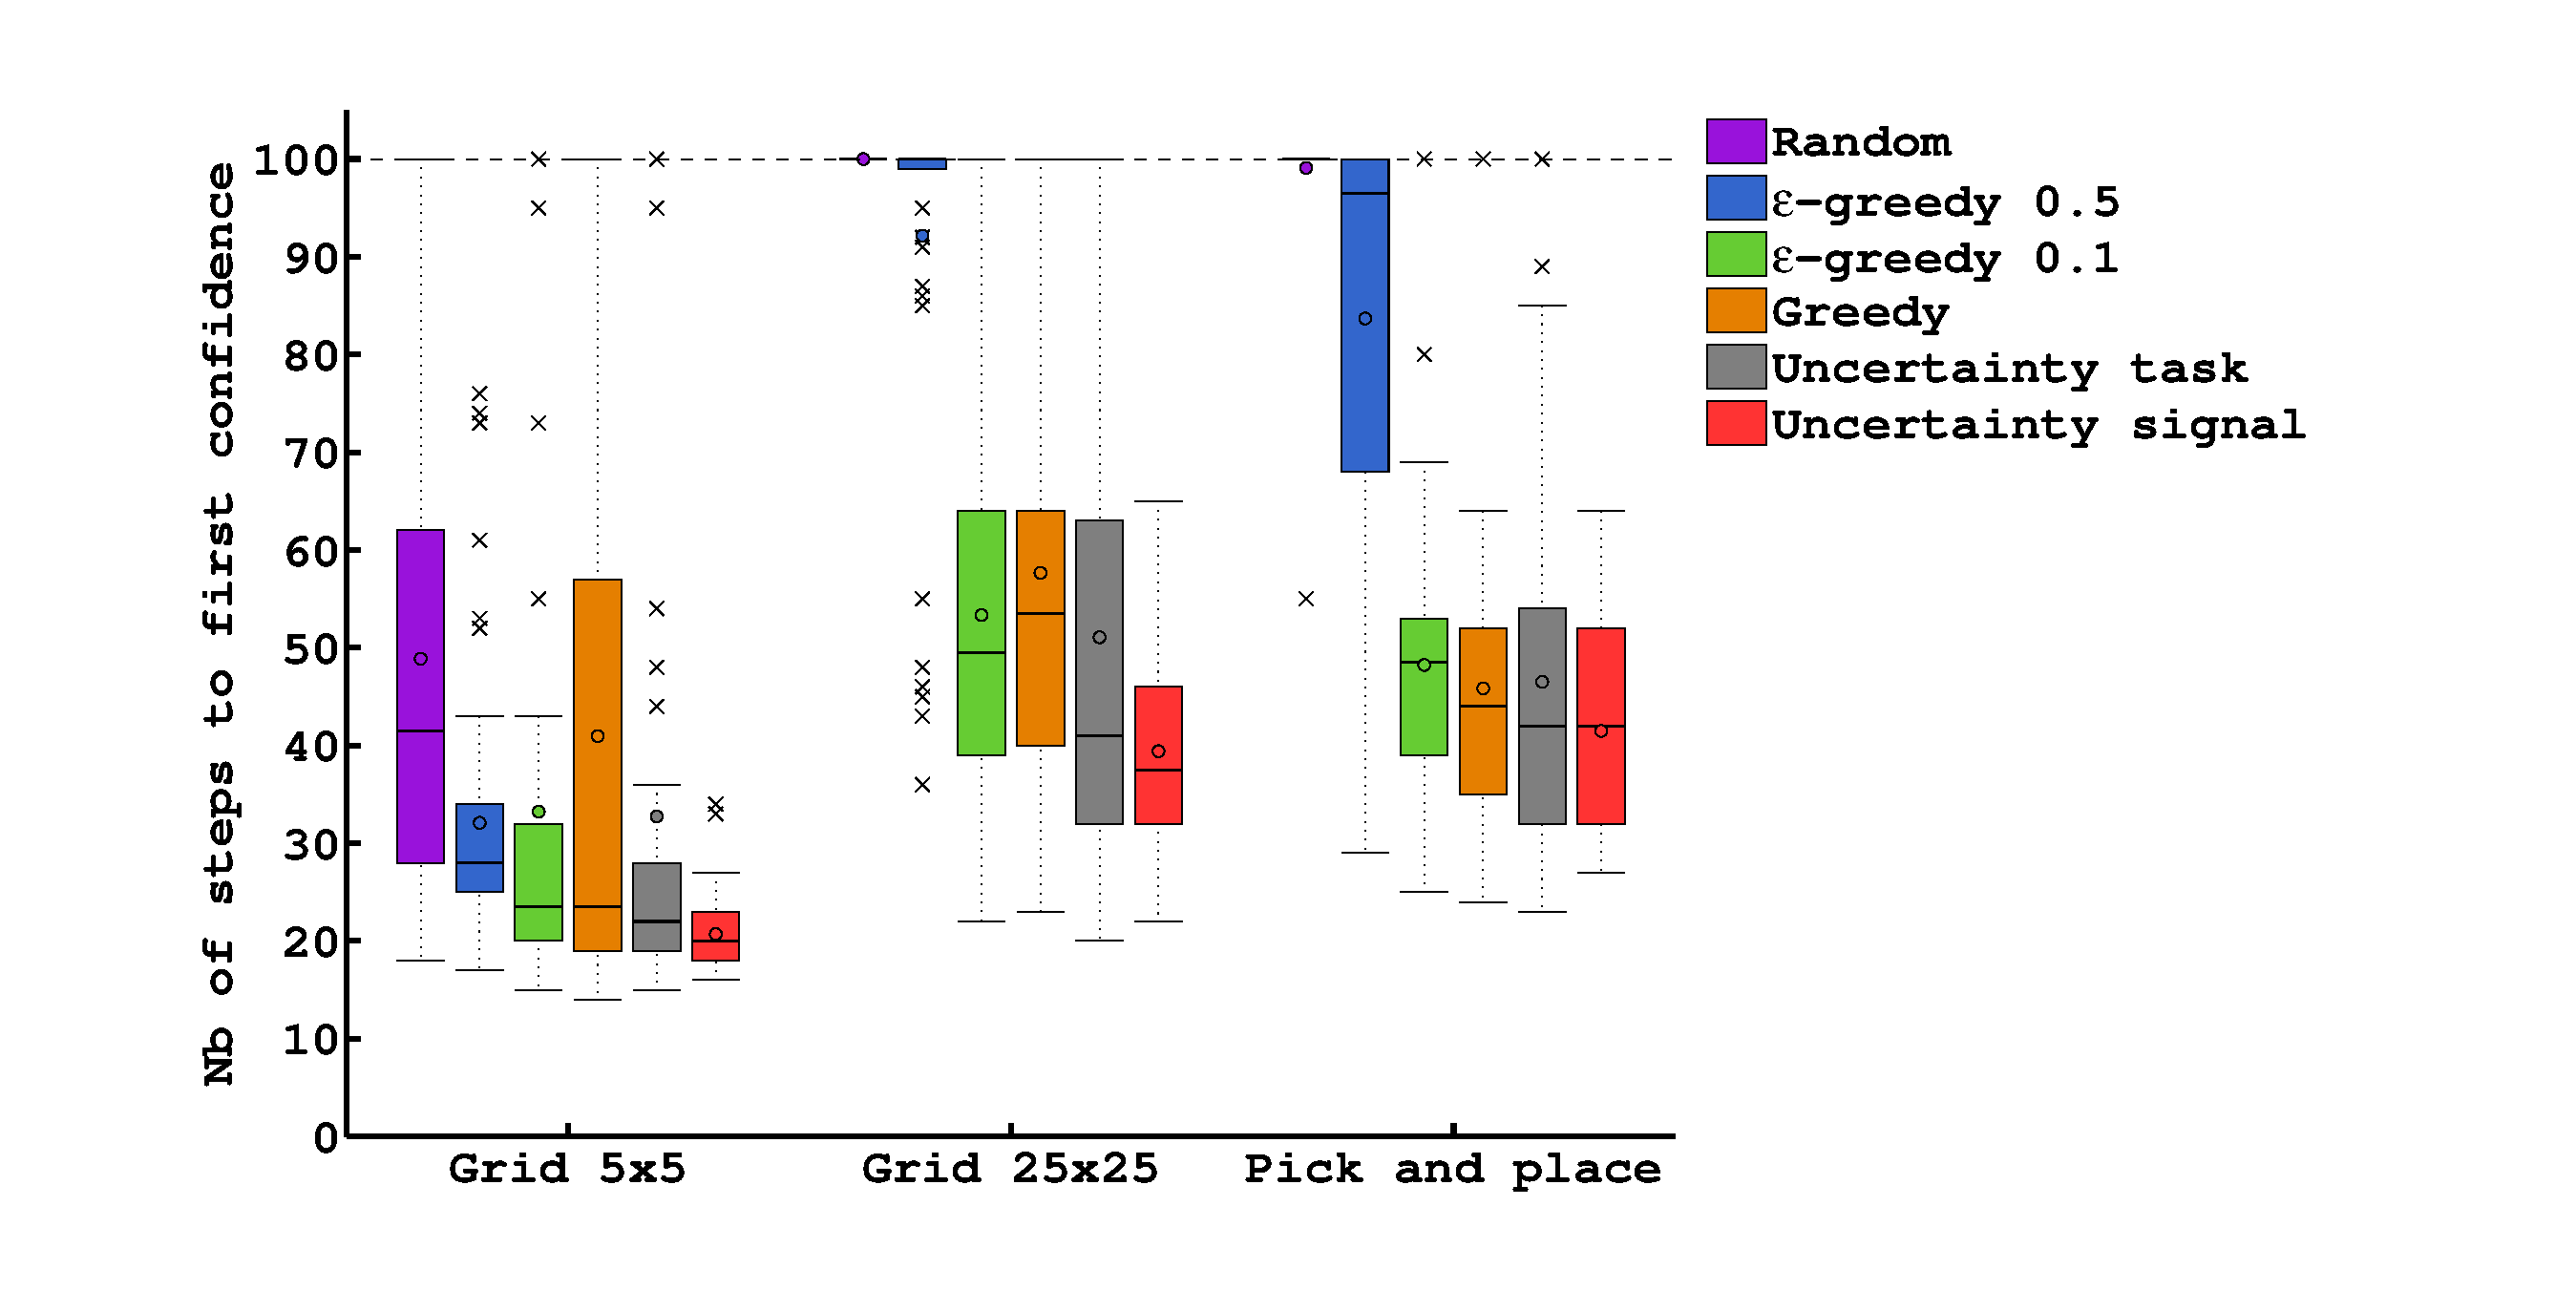
\includegraphics[width=\legendsidesize\columnwidth]{\imgpath/world_properties/firstconfident.eps}
\caption{Number of steps to reach confidence level for the first target.}
\label{fig:wordlpropertiesconfidencefirst}
\end{figure} 

Figure~\ref{fig:wordlpropertiestargetdist} shows the number of actions needed for the agent to reach the goal state once the task is identified with confidence. This plot only considers the runs where a target was reached (see Table~\ref{tab:wordlpropertiesnreach}). For the grid world, all planning methods identify the task less than 5 steps away from its associated goal state. However for the pick and place problem, by following our uncertainty based planning method the agent is on average 10 steps away from the goal state when it identifies a task with confidence.

\begin{figure}[!htbp]
\centering
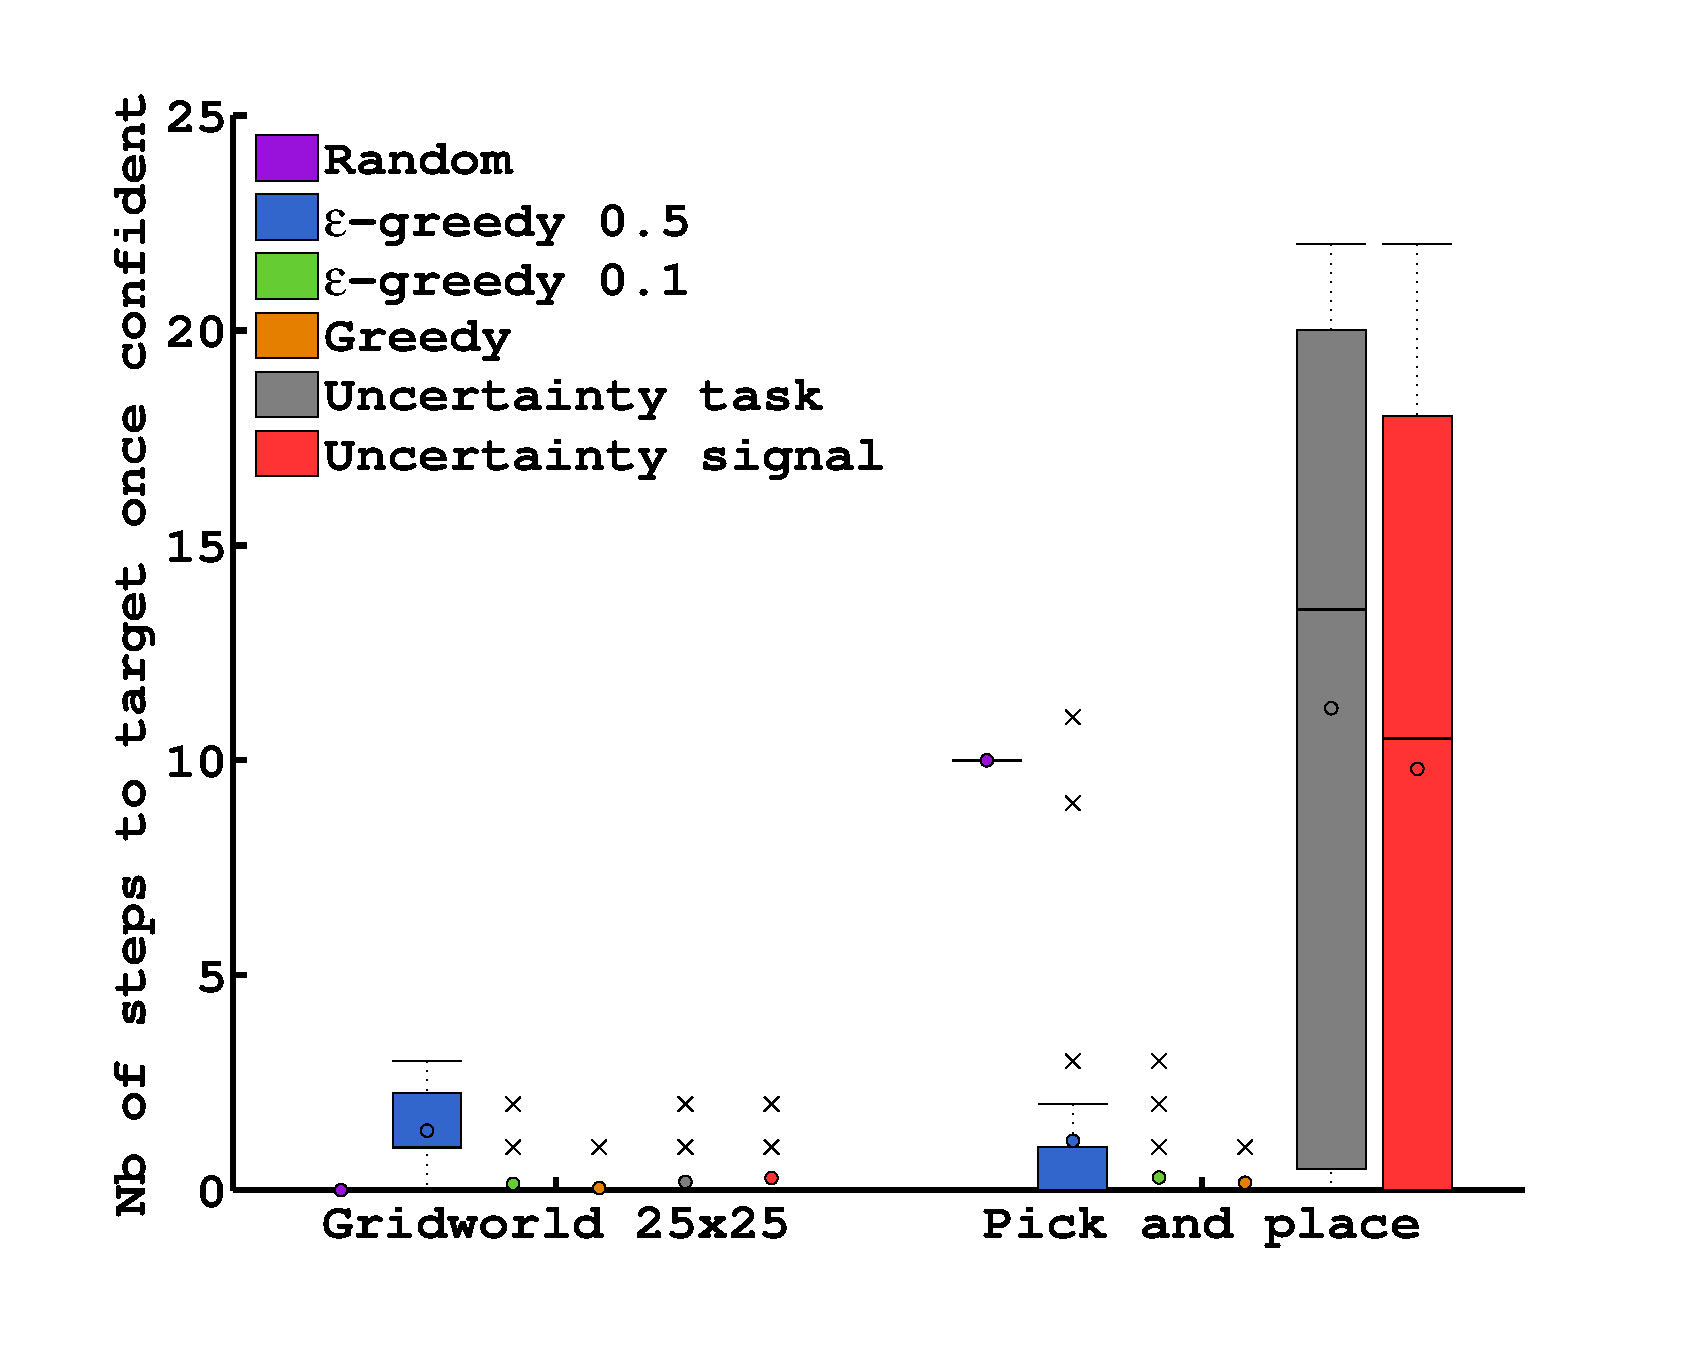
\includegraphics[width=\plotsize\columnwidth]{\imgpath/world_properties/difftargetconfidence.eps}
\caption{Number of actions needed to reach the first target once the agent reached confidence level for this target. This plot only consider the runs where a target was reached in less than 100 steps (see Table~\ref{tab:wordlpropertiesnreach}). Random action selection for the 25x25 grid world is not represented as it never reached any, and random for the pick and place only considers one run.}
\label{fig:wordlpropertiestargetdist}
\end{figure} 

We hypothesized that, given the maze like properties of the pick and place problem, our agent would need to go toward the best hypothesized target states to differentiate between them faster. And therefore that our uncertainty planning method may be more efficient in such case. This hypothesis is not confirmed and requires more investigation on what properties are actually influencing the efficiency of our algorithm and what additional metrics should be considered to improve our strategies. Indeed none of the method presented are considering their performance on the task (yet unknown but estimated) in the action selection process. 

% This is part of the discussion of next subsection.

\todo{We note that the greedy method is going towards the best hypothesis goal state, which confirms our intuition of what is a good planning strategy in such world, but does not explain why our uncertainty method ends-up far from the goal state when the confidence level is reached.}
% In order to explain this differences one should analyze the behavior of the agent and the evolution of the probability associated to each task, and check which group of tasks are ruled out first between the Greedy and the uncertainty based method that may explain the differences of behavior observed.

% Finally, as for the analysis of the size of the worlds, we note that in chapter~\ref{chapter:planning}~and~\ref{chapter:bci} the greedy method shows very poor performances for 30 dimensional signals. Therefore it is required to compare the performances of the planning methods for a variety of datasets with different dimensionality and quality.

\subsection{Discussion}

The main conclusion of this study is that we do not understand well the impact of worlds and datasets properties on the final performance of the system. Many of these properties are tightly linked together and the additional layer of uncertainty inherent to our problem makes the dependencies hard to identify.

However one important aspect highlighted by the study is that our uncertainty measure should be combined with other metrics to optimize additional criteria on the task. Our measure was developed to discriminate faster the correct hypothesis from the set of possible tasks and not to also execute that task as fast as possible.

On this basis, we propose two different types of scenario to investigate: 
\begin{itemize}
\item \textbf{Target based scenarios:} In these scenarios, the goal of the agent is to execute one specific action in a particular state, but in situation where failing the task have bad consequences. 
% In addition, it is important to succeed in the task. and should not make mistakes in the execution of the task. 
Lets consider a robot that should identify one object among a finite set and put it to the bin for a human. The robot can navigate freely around the objects in order to collect feedbacks from the human. However, the robot should only grasp and throw an object once it is confident that it is the object intended by the human. 
% This includes all the scenario considered in this thesis, and as seen in this section there is room to improve over our uncertainty method by including information about the hypothesized task.
This problem is an instantiation of the visual navigation task used in our BCI experiments. In chapter~\ref{chapter:limitations:wordlproperties}, we have seen that our uncertainty method can be outperformed by a simpler method (greedy) when the goal is to identify and perform the task as fast as possible. It is likely that a pure greedy method can be outperformed. The problem with our uncertainty measure was that the robot could disambiguate between task ``far away'' from their respective goal states. Requiring additional steps to reach the correct goal state once identified. A potential avenue is to merge our measure of uncertainty with information about the optimal policy of each task, such that, for two states of equal uncertainty, the state closer to the potential targets is preferred. The resulting problem lies in weighting between seeking for uncertainty reduction and optimizing the position of the agent with respect to the, yet unknown, goal state.

% When all task are equally probable, only the uncertainty should be taken into account. And once there is no more uncertainty, i.e. when confidence is reached, the action should be selected according to the task policy.

\item \textbf{Reward maximization scenarios:} In these scenarios, the goal of the robot is to maximize the cumulative reward associated to the correct task. The problem is that many tasks may have similar reward functions. Therefore it is not always necessary to identify the correct task with confidence to collect maximal rewards. For example, in our puddle word scenario of section~\ref{chapter:limitations:continousstate}, two tasks may share the same goal area but have different areas to avoid. If the robot can reach the shared goal area by avoiding the negative areas of both hypothesis, then the agent will have maximized the collected reward without ever knowing what specific task the user had in mind. In such case, the agent must known whether merging two reward functions is more optimal than trying to differentiate between them.